\section{Internship accomplishments}
\label{sec:accomplish}

This section describes the main tasks achieved during the traineeship, along with the reason why they were needed, the way they have been implemented and the knowledge that they brought.

\subsection{Building of UI components}
\label{ssec:ui_components}

As mentioned in {\sc subsection}~\ref{ssec:frameworks}, ReactJS is based on encapsulated components, most of them appearing several times on the website. They can be very basic (e.g. buttons) or more elaborate (e.g. modals). For this reason, it is a good idea to create a library of generic components, that can be reused as many times as required. This saves a lot of development time, and also assures a certain homogeneity between the different pages of the application.

Several developers, including myself, built this library in a folder named \guillemotleft{} ui \guillemotright{}. One of the components that I have created is the \guillemotleft{} DatePicker \guillemotright{}. Since this is a rather complex component, a good reflex is to first take a look at existing ReactJS plugins. They are usually hosted on Github, with a demonstration link of how they behave and a quick download option via npm.

I found a few possible date pickers, so a selection had to be made, based on several criteria. One of them is the latest update of the repository: if it is quite recent, it means that the owner can quickly help in case there is any problem with the plugin. Also, if the repository has a lot of stars, it means that lots of people using it are satisfied. Another good sign is a low number of open issues in the repository. In the end, the choice was a plugin called \guillemotleft{} react-datepicker \guillemotright{}~\footnote{https://github.com/Hacker0x01/react-datepicker}.

Then, to start the implementation, a \guillemotleft{} DatePicker \guillemotright{} folder was added to the library of components. In this new folder, I created a file named \textit{DatePicker.js} which contains the code of the component. At the top of this file are a few \guillemotleft{} import \guillemotright{} statements, as seen on {\sc figure}~\ref{fig:imports}: ReactJS, the previously downloaded plugin, and also \textit{DatePicker.scss}.

\begin{figure}[H]
    \centering
    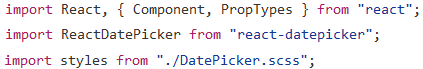
\includegraphics[scale=0.9]{figure/imports.png}
    \caption{The needed importations for the DatePicker UI component.}
    \label{fig:imports}
\end{figure}

This last imported file contains the local CSS styles for the date picker, that will not be used anywhere else in the application. This system makes sure that if changes are made in the CSS for one component, they will not affect other UI elements. However, Konnektid uses some global CSS values (fonts, colors, etc) that are defined in SCSS files at the root of the \guillemotleft{} ui \guillemotright{} folder. Those are meant to be reused in every component, to make the website more harmonious. So I used them to customize react-datepicker, and the final result is presented on {\sc figure}~\ref{fig:datePicker}.

\begin{figure}[H]
    \centering
    
\includegraphics[scale=0.6]{figure/datePicker.png}
    \caption{The final DatePicker presentational component.}
    \label{fig:datePicker}
\end{figure}

This assignment was an efficient way to learn JavaScript and some good ReactJS practices. Moreover, it was a great introduction to the ReactJS community and all the support that it brings, especially with the numerous plugins that are shared.

It is important here to note that the pages that already existed on the website do not use this new library of UI components. Instead of rebuilding them all, which would have been terribly time-consuming, we were able to keep them in separate folders: \textit{public} for public pages such as the homepage, \textit{app} for private pages~\footnote{Pages accessible only when the user is logged in.} such as the activity feed. They are now referred to as \guillemotleft{} old \guillemotright{} pages whereas the most recent pages, built with the UI library, are called \guillemotleft{} new \guillemotright{}.

\subsection{Implementation of new pages}
\label{ssec:new_pages}

It has been explained in {\sc subsection}~\ref{ssec:concept} that Konnektid's main goal for the year is to test and validate their business model, which relies on
professional teachers. This requires the implementation of several new pages and functionalities, and lots have been built during the internship. Among them, one will be described here: the course page.

It refers to the page used by teachers to create, edit and publish a course. It had to be built from scratch, for both desktop and mobile, based on designs
made by Konnektid's former designer. It is now released and used by professional teachers, and a desktop example is visible in {\sc attachment}~\ref{ssec:courseDesktop}.

The page features two main elements:

\textbf{The top section} which contains the main information about the course (picture, title, price\ldots) and the teacher (avatar, name\ldots).
The teacher name is a direct link to his or her profile. This section also provides a button \guillemotleft{} Enroll now \guillemotright{} for the students to book the course.

\textbf{The bottom section} which is divided in two parts. The right part takes most space on the page and gives an in-depth description of the course
(methodology, requirements\ldots). The left part, thinner, shows practical information about the course (format, length\ldots) and another \guillemotleft{} Enroll now \guillemotright{} button with a reminder of the price. Below this are the sharing functionalities: Facebook, Twitter,
email, and WhatsApp on mobile.

The initial step in the implementation was to create the corresponding route, to indicate that \url{www.konnektid.com/course/:id} (where \textit{id} is the course identifier) leads to the \textit{Course} route handler. It is a JavaScript file rendering the \textit{Course} component inside of the website layout. Later on, when the UI is finished and the logic is added using Redux, the route handler renders the \textit{Course} container instead of the component.

To build the \textit{Course} component, the first challenge was to decide how to divide
it in sub-components, each of them implemented in their own folder with local CSS styles. For instance, the biggest bottom part shown on {\sc figure}~\ref{fig:courseDescription} is a component called \guillemotleft{} CourseDescriptionCard \guillemotright{}.

\begin{figure}[H]
    \centering
    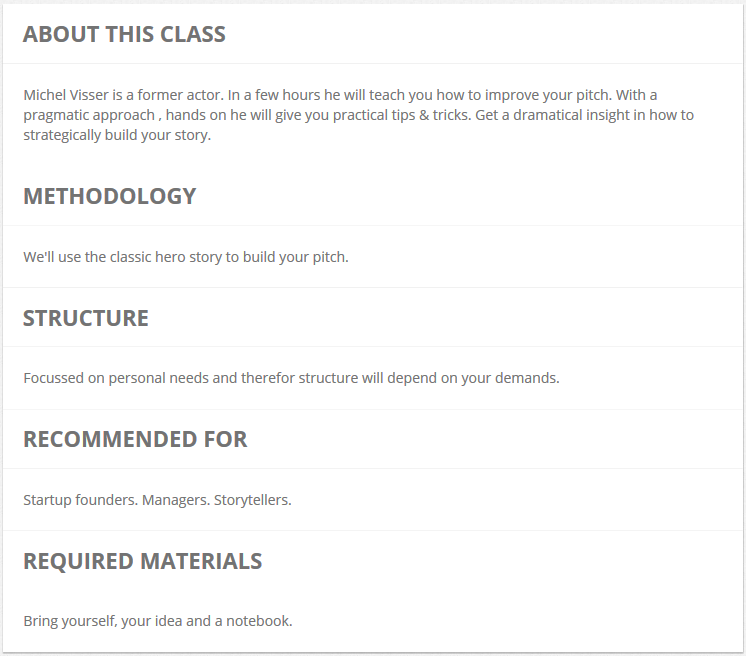
\includegraphics[scale=0.6]{figure/courseDescription.png}
    \caption{An example of course description, in the bottom part of the course page.}
    \label{fig:courseDescription}
\end{figure} 

We can see that it contains several sections, that are similar in presentation and only differ by their title and content. So
it made sense to create a reusable \guillemotleft{} CourseDescriptionItem \guillemotright{} sub-component, to render each of them with title and content passed down as props. This reasoning respects the single responsibility principle previously mentioned in {\sc subsection}~\ref{ssec:frameworks} and avoids duplicated code.
These are two of the many good practices for writing maintainable code~\cite{maintainable}, i.e. code that is easy to read, to modify and to extend.

After the static page had been built, I was asked to add inline editing features to it.
This means that elements can be edited in-place, in the context where they will be published. I used an editor framework for ReactJS called \textit{DraftJS}, which enables the creation of rich content such as bold/italic text or lists of items~\cite{draftJS}. An example of editable CourseDescriptionItem component is displayed on {\sc figure}~\ref{fig:courseEdit}. When mousing over the content, a gray frame appears around it to draw attention, and the teacher can just click on it to start writing as explained by the green tip on top. For now it is empty, so the placeholder \guillemotleft{} If you leave this empty... \guillemotright{} is displayed.

\begin{figure}[H]
    \centering
    
\includegraphics[scale=0.4]{figure/courseEdit.png}
    \caption{One of the course description items in edition mode.}
    \label{fig:courseEdit}
\end{figure}

DraftJS is based on an \guillemotleft{} Editor \guillemotright{} component, whose state is stored in an \guillemotleft{} EditorState \guillemotright{} object holding all the information about the content: the text and its decoration (bold, italic\ldots), the selection state\ldots A method \textit{onChange}, passed down as prop, is called to update the state every time the user changes the content of the editor. Moreover, it is possible to define customized key bindings for the editor, by using the \textit{keyBindingFn} and \textit{handleKeyCommand} props. The first function returns a command string depending on the pressed key, then the second one takes that string as input and outputs the corresponding changes on the editor state.

This page was the first static page I fully created, and it made me realize how useful the components library mentioned in {\sc subsection}~\ref{ssec:ui_components} is. It was also a great occasion to improve my skills in JavaScript and SCSS, and to get even more familiar with ReactJS and its derivatives.

\subsection{Refactoring of existing pages}
\label{ssec:refactor}

To include the new features, some old pages of the application had to be modified, usually with small changes: for example, I updated the professional teachers presented on the homepage, in the \guillemotleft{} Book a professional teacher \guillemotright{} section. In this case, revising the former code was enough. But sometimes, a whole refactoring was needed, and in that case the best option is to entirely rebuild the page using the UI library. 

This is what happened for the teachers landing page, describing Konnektid's offer for professional teachers in order to convince people to become one. It was decided to improve it because the conversion rate (i.e. the number of users signing up as teachers compared to the number of visitors of the page) obtained via the analytics was not satisfying. 

To get started, we had a brainstorm session to determine what contents were needed, and how they should be structured. We came up with a wireframe\footnote{Basic skeleton of the page, representing the main UI elements and how they work together.}, and since there was no designer back then, this was the only support I had for development. So I quickly built and presented a first draft, to make sure I was heading the right way and to get a first round of feedback.

Based on this, I could iterate the process and gradually improve the interface until it was validated, for both desktop and phone. Then, to verify that we were sending the right message, the copywriting was reviewed together with the community manager. She also helped me out by collecting quotes from current professional teachers, who were then integrated in the page as social proof of the concept. This first version was released in \textit{alpha}. A while later, a designer joined the team and suggested a few modifications concerning the User Experience (UX) and the UI of the page, so we worked together on improving it. 

In the meantime, the registration process for professional teachers was also being refactored, but it was not yet ready. So I had to implement a temporary sign-up flow, based on the former one visible on {\sc figure}~\ref{fig:signUpFlow}.

 \begin{figure}[H]
    \centering
    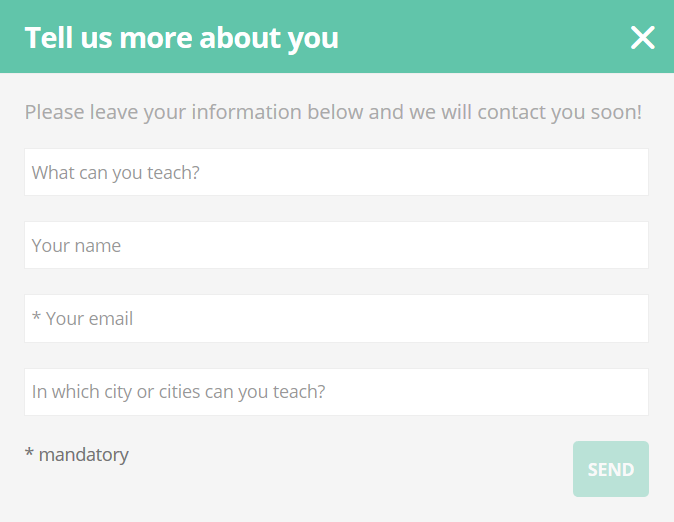
\includegraphics[scale=0.6]{figure/signUpFlow.png}
    \caption{The registration form for professional teachers.}
    \label{fig:signUpFlow}
\end{figure}

It is a modal with four fields to fill in: the name and email of the applicant, the skill(s) to teach, and the city or cities where he/she could teach. When clicking on \guillemotleft{} Send \guillemotright{}, an email is sent to the Konnektid team with all the provided information. If everything goes well, a new screen appears to indicate the success, and the request can be treated by Konnektid (i.e. get in touch with the person, verify the certifications\ldots). If there is a problem (for instance while sending the email), an error screen appears to inform the applicant that the request could not be sent.

I had to re-create this modal with the UI components of the new library, as a component called \guillemotleft{} BecomeTeacherModal \guillemotright{}. It contains a form, \guillemotleft{} BecomeTeacherForm \guillemotright{}, receiving the screen as prop, which can have three values: \guillemotleft{} form \guillemotright{}, \guillemotleft{} success \guillemotright{} or \guillemotleft{} error \guillemotright{}. It also has a container to manage the state of the modal (i.e. when to show it or not) and of the form (i.e. which screen to display) thanks to a Redux reducer that I implemented along with its tests. The form itself was built with \textit{redux-form}, a plugin specially designed for managing form state in React using Redux.

I used \textit{redux-form} in the container on top of the BecomeTeacherForm component, to perform all the necessary verifications needed to validate the form. For example, the email address is mandatory, and also needs to respect a certain format (e.g. test@test.com). The code of the BecomeTeacherForm container, testing the email value, can be seen on {\sc figure}~\ref{fig:reduxForm} where \textit{isEmail} is a utility checking the email format.

 \begin{figure}[H]
    \centering
    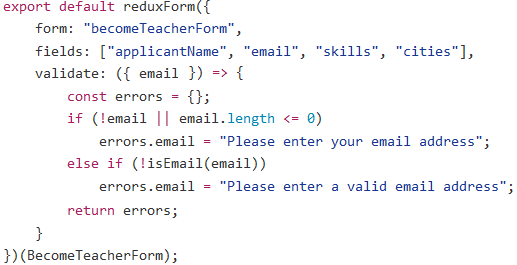
\includegraphics[scale=0.8]{figure/reduxForm.png}
    \caption{The \guillemotleft{} BecomeTeacherForm \guillemotright{} container.}
    \label{fig:reduxForm}
\end{figure}

Then, the error to display (if any) and the validation of the email can be used in the component via \textit{email.error} and \textit{email.valid}. The error will appear in red under the corresponding input, to inform the user that something is wrong. The validation is used to able or not the \guillemotleft{} Send \guillemotright{} action, as on {\sc figure}~\ref{fig:signUpFlow} where the empty email field disables the button.

The remaining task for this project was to create a GraphQL mutation to send the request email to Konnektid. I did not have time to complete the email, but I implemented \textit{notifyRegisteredTeacherMutation.js} which takes as input a \guillemotleft{} TeacherRegistration \guillemotright{} object containing all the fields of the form. When \guillemotleft{} Send \guillemotright{} is clicked, the mutation is called in the \textit{becomeTeacherModal} reducer, via the \textit{completeRegistrationProcess} method visible on {\sc figure}~\ref{fig:completeRegistration}.

 \begin{figure}[H]
    \centering
    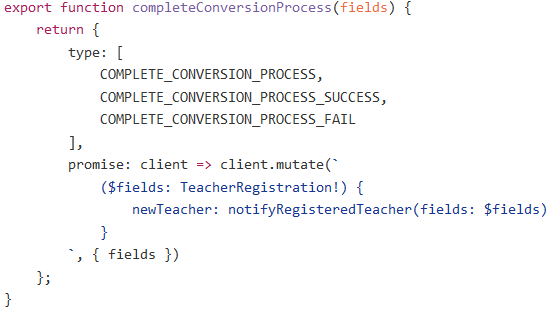
\includegraphics[scale=0.8]{figure/completeRegistration.png}
    \caption{The function handling the registration request.}
    \label{fig:completeRegistration}
\end{figure}

This asynchronous function fires the \textit{COMPLETE\_REGISTRATION\_PROCESS} action, and if the mutation is successful sends \textit{COMPLETE\_REGISTRATION\_PROCESS\_SUCCESS} which updates the screen to \guillemotleft{} success \guillemotright{}. Otherwise, \textit{COMPLETE\_REGISTRATION\_PROCESS\_FAIL} is returned and the screen becomes \guillemotleft{} error \guillemotright{}.

The final desktop version of the new teachers landing page is available in {\sc attachment}~\ref{ssec:teachersPage}. It was great to follow the creation process from A to Z, and to be fully responsible for it, even if it was challenging to build everything from scratch with technologies I had never used before.

\subsection{New navigation}
\label{ssec:new_nav}

After discussions with the designer, it appeared that the navigation in the private pages of the application was unclear and too complicated. So, it has been decided to refactor it, and I took care of the implementation (both in mobile and desktop) based on design mockups. I will only describe the process for the old pages, as the one for new pages is basically the creation of UI components, and it is already detailed in {\sc subsection}~\ref{ssec:ui_components}.

First, since this is a consequent change, I created a feature flag (trick described in {\sc subsection}~\ref{ssec:env}) named \textit{new\_navigation\_enabled}. I set it to true in the \textit{development} and \textit{alpha} configuration files, but to false in \textit{production}. This means that no matter what happens, the changes will only appear in \textit{alpha} and will not affect \textit{production} (the actual website). I also added it to \textit{legacyConfig.js}, visible on {\sc figure}~\ref{fig:legacyConfig}, which takes the configuration for new pages and converts it into configuration for old pages.

\begin{figure}[H]
    \centering
    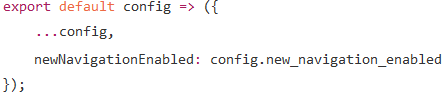
\includegraphics[scale=0.8]{figure/legacyConfig.png}
    \caption{The content of \textit{legacyConfig.js}.}
    \label{fig:legacyConfig}
\end{figure}

This configuration can then be passed down to components as \guillemotleft{} config \guillemotright{} prop, thanks to a helper called \textit{connectLegacyConfig}. The feature flag is then accessed via \textit{this.props.config.newNavigationEnabled} and needs to be checked at every code modification, to be certain that changes will be applied only if the flag is set to true.

Since it is usually difficult to dive into existing code and modify it, especially if somebody else wrote it, I started by updating the old pages. This code is not as structured as the one for new pages, because it does not use presentational components nor local CSS styles. Instead, it features a lot of stateful components, and global CSS files stored in a separate \guillemotleft{} styles \guillemotright{} folder, and this made the task really harder. 

In desktop, I thought that the changes would be quite fast to make as the former header ({\sc figure}~\ref{fig:oldNavDesktop}) was relatively similar to the new one ({\sc figure}~\ref{fig:newNavDesktop}). But it turned out to be more complex than expected.

\begin{figure}[H]
    \centering
    
\includegraphics[scale=0.3]{figure/oldNavDesktop.png}
    \caption{The former private header for desktop.}
    \label{fig:oldNavDesktop}
\end{figure}

\begin{figure}[H]
    \centering
    
\includegraphics[scale=0.47]{figure/newNavDesktop.png}
    \caption{The refactored private header for desktop.}
    \label{fig:newNavDesktop}
\end{figure}

The old header was generated based on \textit{private-menu.js}, a file containing all its elements shaped as objects with two fields: the label to display (e.g. \guillemotleft{} My requests \guillemotright{}) and the associated URL (e.g. \guillemotleft{} /requests \guillemotright{}). I had to rebuild this file, as \textit{new-private-menu.js}, to remove unused sections and to include the icons, found in the Font Awesome library~\footnote{http://fontawesome.io/icons/}. So I added to each object a field called \guillemotleft{} icon \guillemotright{}, as seen on {\sc figure}~\ref{fig:icon}. 

\begin{figure}[H]
    \centering
    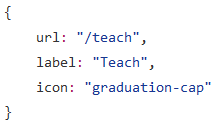
\includegraphics[scale=0.9]{figure/icon.png}
    \caption{An object of \textit{new-private-menu.js}.}
    \label{fig:icon}
\end{figure}

The icon itself is then defined for each menu item in a span, by setting its className property (i.e. its CSS styles) as pictured on {\sc figure}~\ref{fig:classnames}, using a utility called \textit{classnames}~\footnote{https://github.com/JedWatson/classnames} (\guillemotleft{} cn \guillemotright{} on the picture). This method takes several CSS classes, and blends them into one, sometimes under certain conditions. Here for instance, it combines \guillemotleft{} fa \guillemotright{} which refers to the Font Awesome library, \guillemotleft{} fa-lg \guillemotright{} which defines the size of the icon, and \guillemotleft{} fa-\$\{item.icon\} \guillemotright{} which indicates the icon to display (e.g. \guillemotleft{} fa-graduation-cap \guillemotright{} for the object on {\sc figure}~\ref{fig:icon}). 

\begin{figure}[H]
    \centering
    
\includegraphics[scale=0.9]{figure/classnames.png}
    \caption{The definition of the menu icons.}
    \label{fig:classnames}
\end{figure}

Once this was done, I had to implement the \guillemotleft{} My activities \guillemotright{} header section, and its dropdown visible on {\sc figure}~\ref{fig:newNavDesktop}. I created a new component for it (\guillemotleft{} KndActivitiesMenu \guillemotright{}) and a CSS class (\guillemotleft{} activities-menu \guillemotright{}) to place it relatively to the last header section. This also involved a few changes in the last section's CSS class (\guillemotleft{} navatar-menu \guillemotright{}). The activities menu was then included inside the \guillemotleft{} KndPrivateHeader \guillemotright{} component, as seen on {\sc figure}~\ref{fig:activitiesImpl}, where \textit{renderActivitiesMenu()} renders the \guillemotleft{} KndActivitiesMenu \guillemotright{} component.

\begin{figure}[H]
    \centering
    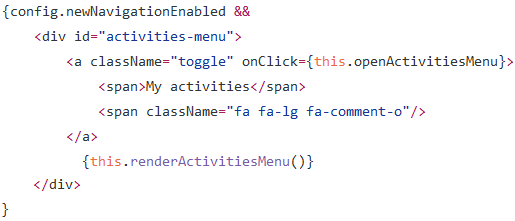
\includegraphics[scale=0.9]{figure/activitiesImpl.png}
    \caption{The implementation of the activities menu.}
    \label{fig:activitiesImpl}
\end{figure}

Finally, \guillemotleft{} KndPrivateHeader \guillemotright{} is stateful, and handles by itself the logic of showing (or not) the dropdowns it contains. It already had in its state a variable named \guillemotleft{} showProfileMenu \guillemotright{}, used to handle the profile dropdown. This variable is updated by calling either \textit{closeProfileMenu()} or \textit{openProfileMenu()}, fired when clicking on the user's name. To be able to toggle the new activities menu, I extended the state with \guillemotleft{} showActivitiesMenu \guillemotright{}, and implemented the related methods \textit{closeActivitiesMenu()} and \textit{openActivitiesMenu()}.

After updating the desktop navigation, I worked on the mobile one (still in old pages). This time, it was completely different from the old version: it used to be a burger button on the top left, toggling an offcanvas menu with all the possible sections. Now it is a header with full-width dropdowns, visible on {\sc figure}~\ref{fig:newNavPhone}. I thought this would be harder to implement than the desktop version, but in the end it was actually faster because it did not involve a lot of modification in the code, but mainly addition.

\begin{figure}[H]
    \centering
    
\includegraphics{figure/newNavPhone.png}
    \caption{The new private navigation for phone.}
    \label{fig:newNavPhone}
\end{figure}

First, I created a static version, without the dropdowns, and its corresponding CSS class (\guillemotleft{} mobile-main-menu \guillemotright{}). It was then integrated to \guillemotleft{} KndPrivateHeader \guillemotright{} via \textit{renderMobileHeader()}, with a previous check of the flag, similarly to the desktop activities menu previously described.

Then, I built the dropdowns, respectively rendered in \guillemotleft{} KndPrivateHeader \guillemotright{} via \textit{this.renderMobileActivitiesMenu()} and \textit{this.renderMobileProfileMenu()}. Since they both show up full-width under the header, I created a wrapper CSS class for them (\guillemotleft{} mobile-menu-wrapper \guillemotright{}) to define this behavior. Finally, I had to expand the state again, by adding the \guillemotleft{} showMobileProfileMenu \guillemotright{} and \guillemotleft{} showMobileActivitiesMenu \guillemotright{} variables, along with writing their corresponding opening and closing functions. 

I was responsible for this new navigation project, which means that I had to keep the other developers informed of the progress by regular status updates. Once it was finished, I was asked to setup a demonstration for it, so that the whole team could see it and give feedback. Unfortunately, the feedback was not always positive, and some of the changes had to be reversed. For the developers team, it was a reminder that we should always validate the mockups with the rest of the team before implementing them. Personnally, this experience taught me to take responsability for the code I produce, and to accept critics on it despite the time spent to write it.

\subsection{Analytics}
\label{ssec:analytics}

Another assignment of the internship was to work on improving the web analytics, that are a precious help for testing the new features and proving the business model. I got to implement them in both old and new pages.

For the new pages, such as courses, the implementation has already been detailed in {\sc section}~\ref{sec:analytics} so I will just briefly describe my contribution. For reminder, analytics there use Redux actions with a type to determine what event to fire, and data to provide required information if any. First, I created all needed action creators, to build the necessary actions with explicit types and relevant data. Then, I had to link these to Google Analytics and Mixpanel, by implementing the \textit{mapActionsToAnalytics} that have been shown on {\sc figure}~\ref{fig:mapActions}. 

Sometimes, analytics need to be improved in old pages, usually when adding a supplementary button. This has been the case when I added an \guillemotleft{} Invite friends \guillemotright{} call-to-action (\guillemotleft{} CTA \guillemotright{}) and a little motivation text after a member offered to teach somebody (screen on {\sc figure}~\ref{fig:afterOffer}).

\begin{figure}[H]
    \centering
    
\includegraphics[scale=0.8]{figure/afterOffer.png}
    \caption{The screen appearing after making an offer, now with an \guillemotleft{} Invite friends \guillemotright{} button.}
    \label{fig:afterOffer}
\end{figure}

Konnektid wanted to track the clicks on this new CTA, to compare its performance to the other \guillemotleft{} Invite friends \guillemotright{} buttons dispatched on the website. 

So, I had to figure out how the analytics are fired in the old pages, as they do not have Redux. Instead, a helper called \textit{connectAnalytics} is used to pass down the \textit{analytics} prop to the component that is then accessed via \textit{getAnalytics()}. This prop contains a certain number of functions, each one corresponding to a possible event. In this case I used an existing one, \textit{inviteFriendsClicked}. It takes as parameter a constant representing the source of the event, i.e. from where in the application it has been fired. The possible values for this constant are defined inside the \guillemotleft{} constants \guillemotright{} folder, in \guillemotleft{} InviteFriendsConstants.js \guillemotright{}. This file contains all possible sources for the \guillemotleft{} Invite friends \guillemotright{} event, so I added AFTER\_OFFER to it, as visible on {\sc figure}~\ref{fig:inviteFriendsConstants}.

\begin{figure}[H]
    \centering
    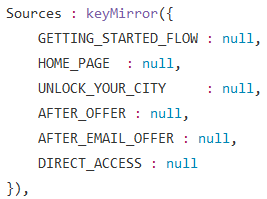
\includegraphics[scale=0.9]{figure/inviteFriendsConstants.png}
    \caption{All the possible sources for the \guillemotleft{} Invite friends \guillemotright{} event.}
    \label{fig:inviteFriendsConstants}
\end{figure}

I could then define \textit{inviteClicked()} ({\sc figure}~\ref{fig:inviteClicked}), which is fired every time a user clicks on \guillemotleft{} Invite friends \guillemotright{} after making an offer, and sends the corresponding analytics. 

\begin{figure}[H]
    \centering
    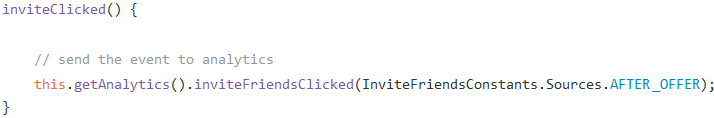
\includegraphics[scale=0.9]{figure/inviteClicked.png}
    \caption{The \textit{inviteClicked()} method, used to send analytics.}
    \label{fig:inviteClicked}
\end{figure}

In addition to the technical learnings, this internship has been a great occasion to dive into startup life and to discover the process of company building. This requires a solid project management system, and the one used at Konnektid is explained in {\sc section}~\ref{sec:management}.